\documentclass[12pt]{article}
\usepackage[utf8]{inputenc}
\usepackage[russian]{babel}
\usepackage{cmap}
\usepackage{amsfonts}
\usepackage{amsmath}
\usepackage{amsthm}
\usepackage{authblk}
\usepackage{cite}
\usepackage{graphicx}
%\usepackage{MnSymbol}
\usepackage{float}
%\usepackage{makecell}
\usepackage{multirow}
%\pagestyle{empty}
\usepackage[]{algorithm2e}
\usepackage[left=2cm,right=2cm,
    top=1cm,bottom=2cm,bindingoffset=0cm]{geometry}

\theoremstyle{definition}
\newtheorem{definition}{Definition}
\newtheorem{restrict}{Restriction}
\newtheorem{proposition}{Proposition}
\newtheorem{consequence}{Corollary}

\theoremstyle{plain}
\newtheorem{statement}{Утверждение}
\newtheorem{lemma}{Лемма}
\newtheorem{theorem}{Теорема}
 

\begin{document}

\thispagestyle{empty}
\begin{center}
\Large Московский государственный университет \\ имени М.В. Ломоносова \\
\Large Механико-математический факультет \\
\Large Кафедра математической теории \\ интеллектуальных систем

\vspace{100pt}

\Large Оценка максимума правдоподобия параметров прямоугольнообразных распределений 
в гауссовском случае \\
\Large Maximum likelihood estimation of the parameters of the 
rectangular-shaped distributions in the Gaussian case

\vspace{20pt}

\Large Курсовая работа \\ Нерсисяна Степана Ашотовича \\ 507 группа
\end{center}

\vspace{50pt}
\begin {flushright}
\Large Научный руководитель: \\
\Large старший научный сотрудник \\ кафедры математической \\ теории интеллектуальных систем \\
\Large к.ф.-м.н. Галатенко Алексей Владимирович
\end {flushright}

\vspace{120pt}

\begin{center}
\Large Москва, 2020
\end{center}

\newpage

\section{Введение}
Параметрические семейства непрерывных распределений используются
в огромном числе приложений для моделирования различных случайных 
величин. При этом семейство распределений зачастую выбирается с
использованием принципа максимума энтропии, так, нормальное распределение
обладает наибольшей энтропией среди всех непрерывных распределений 
на числовой прямой с фиксированным математическим ожиданием и дисперсией \cite{Murphy2013},
в связи с чем активно используется в огромном количестве приложений. Например,
в большом количестве исследований постулируется нормальность распределения
экспрессии генов в гомогенной выборке образцов, хотя такой подход может
подвергаться критике \cite{Hebenstreit2011}. Более очевидным примером является равномерное 
распределение на отрезке $[a, b]$, содержащее в себе наибольшую 
``неопределенность'' среди всех распределений с тем же носителем.

Однако, использование равномерного распределения в приложениях затрудняется
его нерегулярностью, в частности, зависимостью носителя от 
параметров распределения. Для борьбы с этим явлением можно использовать
распределения, плотность которых является приближением к 
плотности равномерного распределения с носителем,
совпадающим со всей числовой прямой. Примером такого приближения 
может служить обобщенное нормальное распределение \cite{Mahesh1989}. 

К сожалению использование такого подхода не решает проблему
абсолютной неустойчивости равномерного распределени к выбросам
в данных. Для борьбы с этим явлением в работе \cite{Pelleg2001} было предложено 
семейство распределений, полученное с помощью ``пришивания'' 
хвостов нормального распределения к равномерной плотности. Авторы
использовали свое распределение для решения задачи кластеризации,
применяя технику разделения смеси распределений с помощью
EM-алгоритма. Однако, в работе не сформулированы алгоритмы, 
выполение которых гарантированно приводит к глобальному максимуму
функции правдоподобия. Более того, параметр, 
отвечающих за ширину нормальных хвостов, считался фиксированным.

В настоящей работе приводится обобщение данной конструкции 
(прямоугольнообразные распределения) и
эффективный алгоритм для поиска глобального максимума 
функции правдоподобия в случае нормальных хвостов. Параметрами
оптимизации являются не только границы отрезка равномерности, но и размер
хвостов распределения. Также приведены результаты вычислительных 
экспериментов, демонстрирующие состоятельность алгоритма.


\section{Построение распределения}

Рассмотрим функцию
$$
k(x | l, h) = \max(0, x - h) - \max(0, l - x)
$$
при $h \geq l$, см. Рис. \ref{k} для примера. Будем использовать ее, чтобы 
``расширить'' моду некоторого распределения, получив плотность, форма которой 
близка к прямоугольнику. А именно, рассмотрим распределение, заданное четной 
плотностью $q(x | \alpha)$, где $x \in \mathbb{R}$ и $\alpha$ -- набор параметров.
Подстановка функции $k$ в аргумент $q$ позволяет создать новое 
распределение, имеющее плато на отрезке $[l, h]$ (прямоугольнообразное распределение):
$$
RSD(x | l, h, \alpha) \propto q(k(x | l, h) | \alpha)
$$

\begin{figure}
\centering
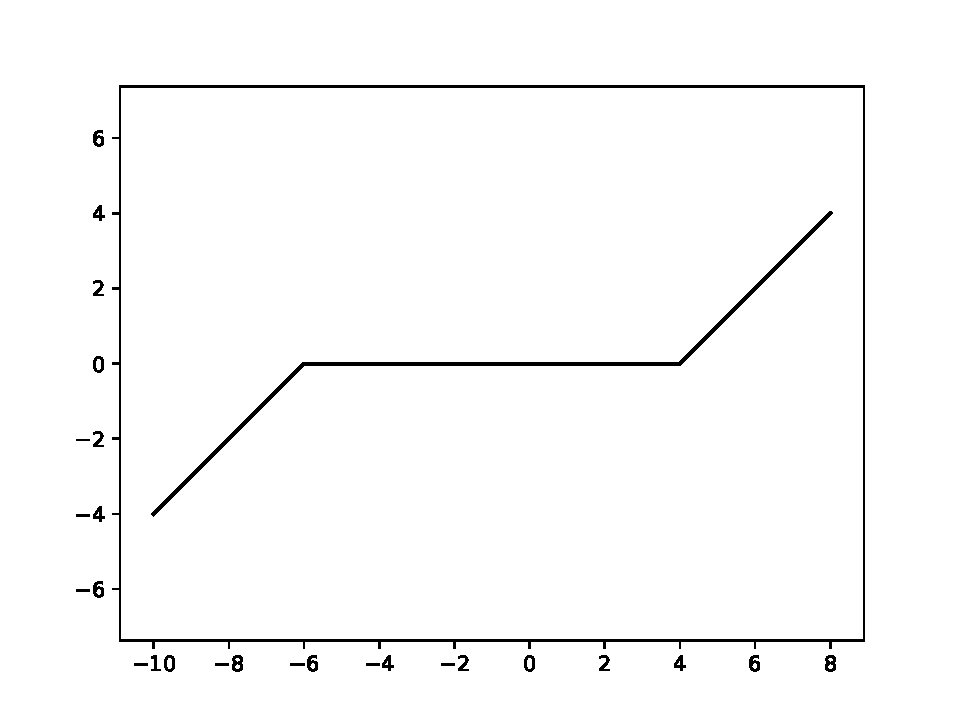
\includegraphics[width=0.6\linewidth]{k.pdf}
\caption{График функции $k(x | l, h)$ при $l = -6,~h = 4$.}
\label{k}
\end{figure}

Для дальнейшей работы с этим распределением необходимо посчитать нормировочную константу:

\begin{align*}
& \int_{-\infty}^{+\infty} q(k(x | l, h) | \alpha) dx = 
 \int_{-\infty}^{l} q(x - l | \alpha) dx + 
\int_{l}^{h} q(0 | \alpha) dx + 
\int_{h}^{+\infty} q(x - h | \alpha) dx = \\
&= 1 + q(0 | \alpha) (h - l)
\end{align*}
Таким образом,
$$
RSD(x | l, h, \alpha) = \frac{1}{1 + q(0 | \alpha) (h - l)} q(k(x | l, h) | \alpha)
$$

\section{Оценка максимума правдоподобия}

Рассмотрим задачу поиска максимума функции правдоподобия для 
прямоугольнообразных распределений. 
Дана выборка $D = (x_1, \ldots, x_N)$, где $x_1 < x_2 < \ldots < x_N$, 
и соответствующие веса $r_1, \ldots, r_N$ (их рассмотрение позволит 
перенести все полученные результаты на M-шаг EM-алгоритма). Нас интересует решение
задачи оптимизации

\begin{align*}
NLL(l, h, \alpha) &= - \sum_{i = 1}^N r_i \log RSD(x_i | l, h, \alpha) = \\
&= \sum_{i = 1}^N r_i \left(
\log \left( 1 + q(0 | \alpha) (h - l) \right) - \log q(k(x_i | l, h) | \alpha)
\right) \rightarrow \min
\end{align*}

Также рассмотрим случай, когда $q$ -- плотность нормального распределения:
$$
q(x | \sigma) = \frac{1}{\sqrt{2 \pi} \sigma} e^{-x^2 / 2 \sigma^2}
$$
Пример графика плотности распределения представлен на Рис. \ref{RSD_normal}

\begin{figure}
\centering
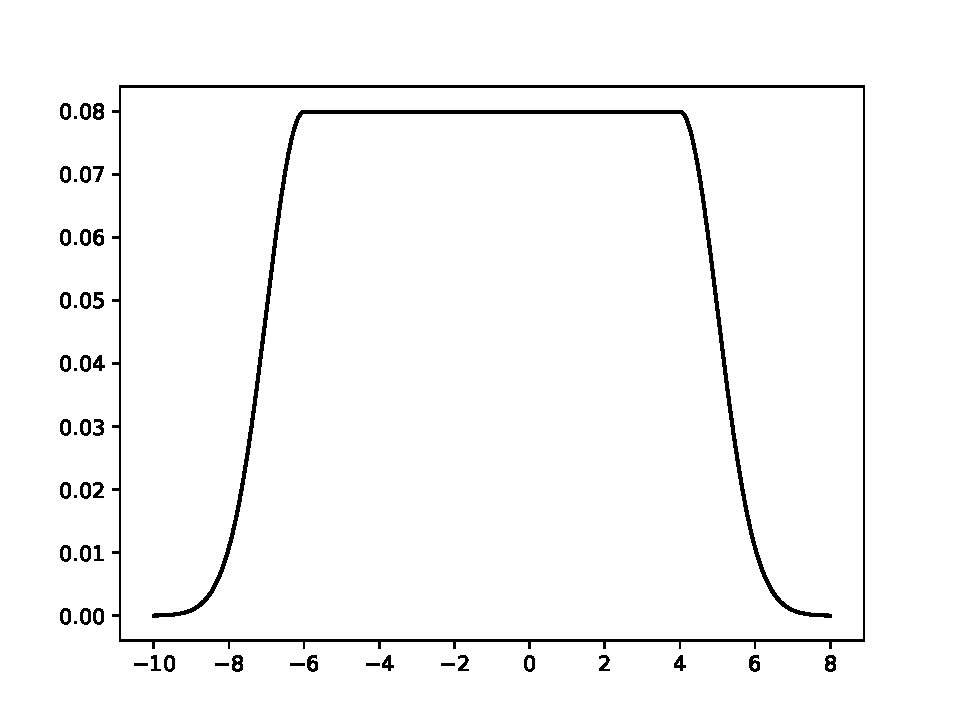
\includegraphics[width=0.6\linewidth]{RSD_normal.pdf}
\caption{График плотности гауссовской $RSD$ при $l = -6,~h = 4,~\sigma=1$.}
\label{RSD_normal}
\end{figure}

Имеем
\begin{align*}
NLL(l, h, \sigma) &=
\sum_{i = 1}^N r_i \left(
\log \left( 1 + \frac{1}{\sqrt{2 \pi} \sigma} (h - l) \right) +
\log \left( \sqrt{2 \pi} \sigma \right) + \frac{k^2(x_i | l, h)}{2 \sigma^2}
\right) = \\
&= r \log \left( \sqrt{2 \pi} \sigma + h - l \right) +
\frac{1}{2 \sigma^2} 
\sum_{i = 1}^N r_i \left( \max(0, x_i - h) - \max(0, l - x_i) \right)^2
\rightarrow \min,
\end{align*}
где
$$
r = \sum_{i = 1}^N r_i
$$

Функцию удобно рассматривать на областях
$$
S_{u,v} = \{l, h: l \leq h, l \in [x_u, x_{u+1}), h \in (x_{v-1}, x_v] \},
$$
где $1 \leq u < v \leq N$ (см. Рис. \ref{regions}); вне объединения этих областей минимум,
очевидно, не достигается. Рассмотрим сужение функции $NLL(l, h, \sigma)$
на область $S_{u,v}$ (для простоты обозначим $NLL$ за $f$):
$$
f(l, h, \sigma) = r \log \left( \sqrt{2 \pi} \sigma + h - l \right) +
\frac{1}{2 \sigma^2} \left(
\sum_{i = 1}^u r_i (l - x_i)^2 + \sum_{i = v}^N r_i (x_i - h)^2
\right)
$$

\begin{figure}
\centering
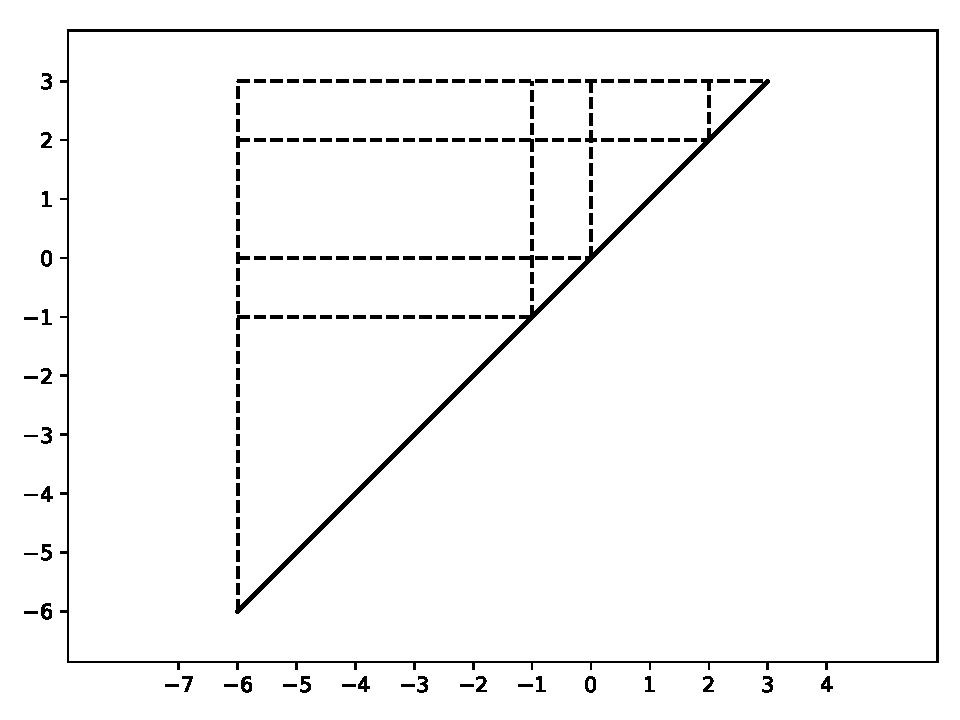
\includegraphics[width=0.6\linewidth]{regions.pdf}
\caption{Области $S_{u,v}$, построенные по выборке $D = \{-6, -1, 0, 2, 3\}$.}
\label{regions}
\end{figure}

Приравняем частные производные функции по $l, h$ к нулю:
\begin{align*}
&\frac{\partial f}{\partial l} = - \frac{r}{\sqrt{2 \pi} \sigma + h - l} +
\frac{1}{\sigma^2} \sum_{i = 1}^u r_i (l - x_i) = 0 \\
& \frac{\partial f}{\partial h} = \frac{r}{\sqrt{2 \pi} \sigma + h - l} -
\frac{1}{\sigma^2} \sum_{i = v}^N r_i (x_i - h) = 0
\end{align*}
Складывая уравнения, получаем:
\begin{equation}
\label{line_equation}
l \sum_{i = 1}^u r_i + h \sum_{i = v}^N r_i =
\sum_{i = 1}^u r_i x_i + \sum_{i = v}^N r_i x_i
\end{equation}
Для удобства введем сокращения:
$$
r^l = \sum_{i = 1}^u r_i,~
r^h = \sum_{i = v}^N r_i,~
x^l = \sum_{i = 1}^u r_i x_i,~
x^h = \sum_{i = v}^N r_i x_i
$$
Тогда уравнение (\ref{line_equation}) принимает вид
\begin{equation}
\label{line_equation2}
r^l l + r^h h = x^l + x^h
\end{equation}

Рассмотрим $u = 1, v = N$. На нем уравнение (\ref{line_equation2}) выглядит как
$$
r_1 l + r_N h = r_1 x_1 + r_N x_N
$$
Точка $l = x_1$, $h = x_N$, очевидно, ему удовлетворяет.
Прямая, выходящая из этой точки, пересекает область 
$S_{1, N}$ либо справа, либо снизу. В случае пересечения справа 
перейдем в область $S_{2, N}$, иначе в область $S_{1, N-1}$.
Лемма \ref{line_intersections} обеспечивает тот факт, 
что прямая, соответствующая новой области, будет проходить
через ту же точку пересечения. В то же время все прямые, ассоциированные с областями 
$S_{1, v}, v < N$ в случае пересечения справа, и прямые, ассоциированные
с областями $S_{u, 1}, u > 1$ в случае пересечения снизу, не будут пересекаться 
со своими областями в силу Леммы \ref{not_intersecting_lemma}. 
Далее, рассуждение повторяется: прямая, соответствующая 
новой области ($S_{2, N}$ или $S_{1, N-1}$) пересекает ее 
границу либо справа, либо снизу. Продолжая процесс движения вправо-вниз 
рано или поздно дойдем до пересечения прямой $l = h$, что соответствует области
$S_{u, v}$, где $v - u = 1$. Таким образом, объединение прямых, 
заданных уравнением (\ref{line_equation2}), по всем областям $S_{u, v}$
определяет ломаную, исходящую из точки $(x_1, x_N)$ и входящую в прямую $l = h$. 
Псевдокод по обходу данной ломаной представлен в Алгоритме \ref{algorithm}.

\begin{algorithm}[H]
\label{algorithm}
\SetAlgoLined
 $u, v \gets 1, N$\;
 $l_{current}, h_{current} \gets x_1, x_N$\;
 $r^l, r^h \gets r_1, r_N$\;
 $x^l, x^h \gets r_1 x_1, r_N x_N$\;
 \While{$v - u \geq 1$}{
  \eIf{$v - u > 1$}{
   $l_{next} \gets \min(x_{u+1}, \frac{x^l + x^h - r^h x_{v-1}}{r^l})$\;
   $h_{next} \gets \max(x_{v-1}, \frac{x^l + x^h - r^l x_{u+1}}{r^h})$\;
  }{
  	$l_{next} \gets \frac{x^l + x^h}{r^l + r^h}$\;
  	$h_{next} \gets \frac{x^l + x^h}{r^l + r^h}$\;
  }
  \eIf{$l_{next} = x_{u+1}$}{
   $r^l \gets r^l + r_{u + 1}$\;
   $x^l \gets x^l + r_{u + 1} x_{u + 1}$\;
   $u \gets u + 1$\;
   }{
   $r^h \gets r^h + r_{v - 1}$\;
   $x^h \gets x^h + r_{v - 1} x_{v - 1}$\;
   $v \gets v - 1$\;
  }
  $l_{current}, h_{current} \gets l_{next}, h_{next}$\;
 }
 \caption{Обход критической ломаной.}
\end{algorithm}

Таким образом, для минимизации функционала достаточно минимизировать 
его на ломаной. Сузим функцию $f$ на звено ломаной:
для этого выразим $h$ из уравнения~(\ref{line_equation2}):
$$
h = \frac{x^l + x^h}{r^h} - \frac{r^l}{r^h} l
$$
Введем обозначения:
\begin{align*}
t &= r^l l - x^l \\
a &= \frac{1}{r^l} + \frac{1}{r^h} \\
b &= \frac{x^h}{r^h} - \frac{x^l}{r^l} \\
c &= \sum_{i = 1}^u r_i x_i^2 + \sum_{i = v}^N r_i x_i^2
- \frac{(x^l)^2}{r^l} - \frac{(x^h)^2}{r^h}
\end{align*}
Тогда по Лемме \ref{calculations} имеем
\begin{align*}
& h - l = -a t + b \\
& \sum_{i = 1}^u r_i (l - x_i)^2 + \sum_{i = v}^N r_i (x_i - h)^2 =
a t^2 + c
\end{align*}
и
$$
g(t, \sigma) = f(l(t), h(t), \sigma) = 
r \log \left( \sqrt{2 \pi} \sigma - a t + b \right) +
\frac{1}{2 \sigma^2} \left( a t^2 + c \right).
$$
Приравняем частные производные по $t, \sigma$ к нулю:
\begin{align*}
&\frac{\partial g}{\partial t} = 
- \frac{r a}{\sqrt{2 \pi} \sigma - a t + b} +
\frac{a}{\sigma^2} t = 0\\
& \frac{\partial g}{\partial \sigma} = 
\frac{\sqrt{2 \pi} r}{\sqrt{2 \pi} \sigma - a t + b} -
\frac{1}{\sigma^3} \left( a t^2 + c \right) = 0
\end{align*}
Сократим в первом уравнении на $a$, после чего домножим его на $\sqrt{2 \pi}$ и сложим
со вторым:
$$
\sqrt{2 \pi} \sigma t = a t^2 + c
$$
С учетом этого преобразуем первое уравнение:
$$
r \sigma^2 = \sqrt{2 \pi} \sigma t - a t^2 + bt = bt + c
$$
Подставляя сюда 
$$
\sigma = \frac{a t^2 + c}{\sqrt{2 \pi} t}
$$ 
получаем
$$
r (a t^2 + c)^2 = 2 \pi t^2 (bt + c)
$$
или
$$
r a^2 t^4 - 2 \pi b t^3 + 2 c (r a - \pi) t^2 + r c^2 = 0
$$

Остается решить данное полиномиальное уравнение 4-й степени, после чего
выбрать точку локального минимума из полученных решений и границ 
соответствующего звена ломаной. Таким образом, весь алгоритм имеет
сложность $O(N)$.

\section{Вычислительные эксперименты}
Алгоритм был реализован в виде класса на языке Python 3. 
Метод был применен к известной выборке данных Iris, содержащей
численные характеристики 150 ирисов.
Оценка максимального правдоподобия была получена для каждой из компонент
данных независимо, см Рис. \ref{iris}. На этих данных видно разнообразие форм,
которые может принимать плотность распределения: от равномерной
(petal width) до нормальной (sepal width) плотностей.

\begin{figure}[H]
\centering
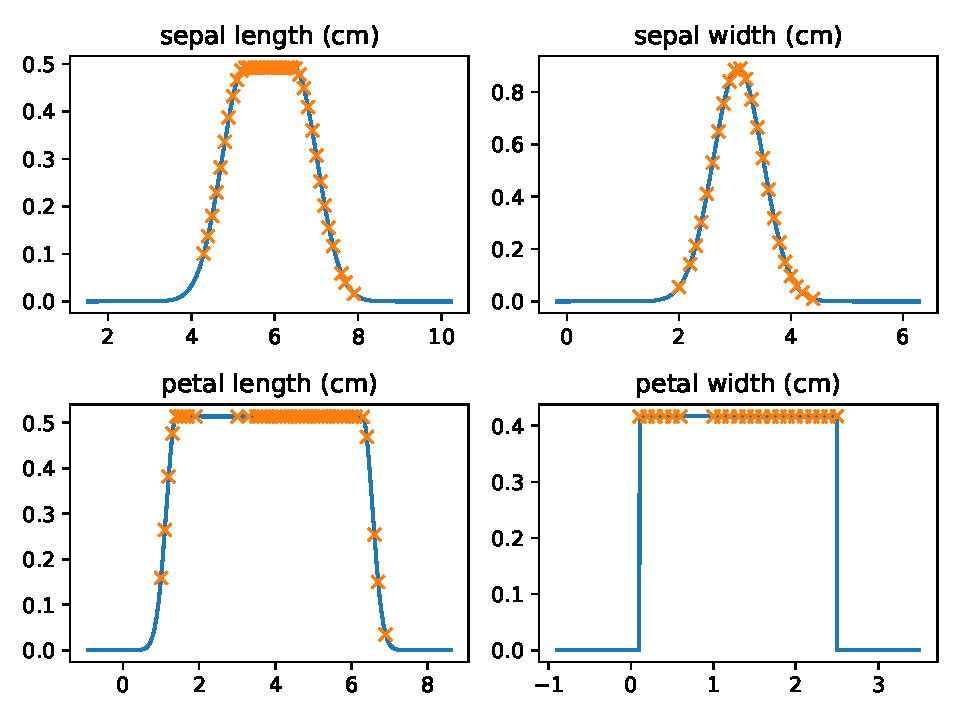
\includegraphics[width=0.6\linewidth]{iris.pdf}
\caption{Оценка максимального правдоподобия для каждой компоненты выборки Iris.}
\label{iris}
\end{figure}


\section{Вспомогательные результаты}

\begin{lemma}
\label{line_intersections}
При $v - u > 1$ верны следующие утверждения:
\begin{enumerate}
\item Прямые, заданные уравнением (\ref{line_equation}) в областях 
$S_{u, v}$ и $S_{u+1, v}$ пересекаются при $l = x_{u+1}$;
\item Прямые, заданные уравнением (\ref{line_equation}) в областях 
$S_{u, v}$ и $S_{u, v-1}$ пересекаются при $h = x_{v-1}$.
\end{enumerate}
\end{lemma}

\begin{proof}
Подставим $l = x_{u+1}$ в уравнение (\ref{line_equation}), записанное для областей
$S_{u,v}$ и $S_{u+1,v}$. Легко видеть, что в обоих случаях получим
$$
h = \frac{\sum_{i = 1}^u r_i (x_i - x_{u+1}) + \sum_{i = v}^N r_i x_i}{\sum_{i = v}^N r_i}.
$$
Аналогично, если подставить $h = x_v$ в уравнение (\ref{line_equation}), записанное для областей
$S_{u,v}$ и $S_{u,v-1}$, получим
$$
l = \frac{\sum_{i = 1}^u r_i x_i + \sum_{i = v}^N r_i (x_i - x_{v-1})}{\sum_{i = 1}^u r_i}.
$$
\end{proof}

\begin{lemma}
\label{not_intersecting_lemma}
Верны следующие утверждения:

\begin{enumerate}
\item Если прямая, заданная уравнением (\ref{line_equation}) в области $S_{u,v}$, проходит
через правую сторону области ($l = x_{u+1}$), то все области
$S_{u, \widetilde{v}}$, где $\widetilde{v} < v$, не имеют пересечений со своей прямой;
\item Если прямая, заданная уравнением (\ref{line_equation}) в области $S_{u,v}$, проходит
через нижнюю сторону области ($h = x_{v-1}$), то все области 
$S_{\widetilde{u}, v}$, где $\widetilde{u} > u$, не имеют пересечений со своей прямой.

\end{enumerate}
\end{lemma}

\begin{proof}
Докажем пункт 1. Из геометрических соображений пересечение прямой с 
правой стороной области означает, что пересечение той же прямой с прямой $h = x_{v-1}$ произойдет
при $l > x_{u+1}$. Применяя лемму \ref{line_intersections} получаем, что прямая, заданная
уравнением в области $S_{u, v-1}$, лежит в некоторой области, расположенной правее, и не 
пересекается с $S_{u, v-1}$ в силу направленности прямой. В силу тех же геометрических 
соображений, прямая, заданная областью $S_{u, v-1}$, пересекается с прямой $h = x_{v-2}$ при
$l > x_{u+2}$. Дальнейшее доказательство проводится повторением рассуждений. 
Пункт 2 доказывается аналогично.
\end{proof}

\begin{lemma}
\label{calculations}
Верны следующие равенства:
\begin{align*}
& h - l = - \left(r^l l - x^l \right) \left(\frac{1}{r^l} + \frac{1}{r^h}\right) +
\frac{x^h}{r^h} - \frac{x^l}{r^l} \\
& \sum_{i = 1}^u r_i (l - x_i)^2 + \sum_{i = v}^N r_i (x_i - h)^2
= \left(r^l l - x^l \right)^2 \left(\frac{1}{r^l} + \frac{1}{r^h}\right) 
+ \sum_{i = 1}^u r_i x_i^2 + \sum_{i = v}^N r_i x_i^2
- \frac{(x^l)^2}{r^l} - \frac{(x^h)^2}{r^h}
\end{align*}
\end{lemma}

\begin{proof}

Доказательство производится прямым вычислением:
\begin{align*}
h - l &= \frac{x^l + x^h}{r^h} - \left(1 + \frac{r^l}{r^h}\right) l =
-r^l l \left(\frac{1}{r^l} + \frac{1}{r^h}\right) + 
x^l \left(\frac{1}{r^l} + \frac{1}{r^h}\right) +
\frac{x^h}{r^h} - \frac{x^l}{r^l} = \\
&= - \left(r^l l - x^l \right) \left(\frac{1}{r^l} + \frac{1}{r^h}\right) +
\frac{x^h}{r^h} - \frac{x^l}{r^l}
\end{align*}

\begin{align*}
& \sum_{i = 1}^u r_i (l - x_i)^2 =
\sum_{i = 1}^u r_i \left(l^2 - 2 l x_i + x_i^2 \right) = 
r^l l^2 - 2l x^l + \sum_{i = 1}^u r_i x_i^2
= \frac{1}{r^l} \left(r^l l - x^l \right)^2
+ \sum_{i = 1}^u r_i x_i^2 - \frac{(x^l)^2}{r^l}
\end{align*}

\begin{align*}
& \sum_{i = v}^N r_i (x_i - h)^2 =
\sum_{i = v}^N r_i \left(
\frac{r^l}{r^h} l - \frac{x^l + x^h}{r^h} + x_i
\right)^2 = \\
&= \sum_{i = v}^N r_i \left(
\left( \frac{r^l}{r^h} l \right)^2 +
\left( \frac{x^l + x^h}{r^h} \right)^2 +
 x_i^2 
-2 r^l l \frac{x^l + x^h}{(r^h)^2}
+2 \frac{r^l}{r^h} l x_i
-2 x_i \frac{x^l + x^h}{r^h}
\right) = \\
&= \frac{(r^l l)^2}{r^h} +
\frac{(x^l + x^h)^2}{r^h} +
\sum_{i = v}^N r_i x_i^2
-2 r^l l \frac{x^l + x^h}{r^h}
+2 \frac{r^l}{r^h} x^h l 
-2 x^h \frac{x^l + x^h}{r^h} = \\
&= \frac{1}{r^h} \left( (r^l l)^2 - 2 r^l l x^l + (x^l)^2 \right) +
\frac{2 x^l x^h + (x^h)^2}{r^h}
-2 x^h \frac{x^l + x^h}{r^h} +
\sum_{i = v}^N r_i x_i^2 = \\
&= \frac{1}{r^h} \left(r^l l - x^l \right)^2
+ \sum_{i = v}^N r_i x_i^2 - \frac{(x^h)^2}{r^h}
\end{align*}

\end{proof}

\begin{thebibliography}{99}
\bibitem{Murphy2013} Murphy KP. Machine learning : a probabilistic perspective. 
Cambridge, Mass. [u.a.]: MIT Press, 2013. 

\bibitem{Hebenstreit2011} Hebenstreit D, Fang M, Gu M, Charoensawan V, van Oudenaarden A, Teichmann SA. RNA sequencing reveals two major classes of gene expression levels in metazoan cells. Mol Syst Biol. 2011 Jun 7;7:497.

\bibitem{Mahesh1989} Mahesh KV, Behnaam A.Parametric generalized Gaussian density estimation. J. Acoust. Soc. Am. 1989 Jun 86;1404.

\bibitem{Pelleg2001} Pelleg D, Moore A. Mixtures of rectangles: Interpretable soft clustering. Proc. 18th International Conf. on Machine Learning. 2001;401-408.

\end{thebibliography}

\end{document}